\newpage
\section{Специальная часть}
\subsection{Обратная динамика}
\label{sec: Обратная динамика}
\pagestyle{fancy}
\fancyhf{}
\rhead{Дипломная работа}
\lhead{Специальная часть}
\rfoot{\thepage}

Чтобы улучшить пилотажные характеристики и точность пилотирования, возможно синтезировать контроллер на основе 
принципа обратной динамики, который показан в работе {\cite{Zoe}}. Но при использовании данного метода порядок числителя будет выше порядка знаменателя, поэтому необходимо использовать фильтры.

В этой работе мы будем вычислять обратную динамику с помощью обратных связей, т.к. здесь нет необходимости ставить дополнительные фильтры.

\subsection{Исслеуемая модель}
\subsubsection{Модель самолёта}

Данная модель была всзята из дисертации {\cite{Diser}}

Основные допущения: 
\begin{enumerate}
    \item Рассмотривается линеаризованная модель короткопериодического движения 
    \item Система исследуется в продольном канале управления
    \item Угол атаки $\alpha$ постоянный и равен $13,7^0$ 
\end{enumerate}

Линейная математическая модель может быть представлена в знакомой форме пространства состояний в виде:
\begin{equation}
    \begin{aligned}
        \dot{x}(t) = Ax(t) + Bu(t) \\
        y(t) = Cx(t) + Du(t)
    \end{aligned}
\end{equation}

Линейная математическая модель может быть представлена в знакомой форме пространства состояний в виде:

\begin{equation}
    \label{eq:Линеаризованная моель СПС}
\begin{bmatrix}
        \dot{V}_x\\ 
        \dot{V}_y\\ 
        \dot{\omega_z}\\ 
        \dot{\theta}
    \end{bmatrix} =
    \begin{bmatrix}
        -0.0110 & 0.0433 & 1.7295 & -7.1876\\ 
        -0.0691 & -0.6975 & -7.0678 & -54.8976\\ 
        0.00011 & 0.00116 & -0.35407 & 0.0911\\ 
        0 & 0 & 1 & 0
    \end{bmatrix} \begin{bmatrix}
        V_x\\ 
        V_y\\ 
        \omega_z \\ 
        \theta
    \end{bmatrix} 
        +\begin{bmatrix}
        -0.4412\\ 
        -12.388\\ 
        -0.58446 \\ 
        0
    \end{bmatrix}  u
\end{equation}

Система ДУ приводит к следующей краткой аэродинамической и управляющей производной:

\begin{equation}
    \label{eq:Линеаризованная моель СПС}
\begin{bmatrix}
        \dot{V}_x\\ 
        \dot{V}_y\\ 
        \dot{\omega_z}\\ 
        \dot{\theta}
    \end{bmatrix} =
    \begin{bmatrix}
        x_{V_x}& x_{V_y}&x_{\omega_z} &x_{\theta} \\ 
        z_{V_x}&z_{V_w} &z_{\omega_z} &z_\theta \\ 
        m_{V_x}&m_{V_y} &m_{\omega_z} &m_\theta \\ 
        0& 0& 1&0 
    \end{bmatrix} \begin{bmatrix}
        V_x\\ 
        V_y\\ 
        \omega_z \\ 
        \theta
    \end{bmatrix} 
        +\begin{bmatrix}
        x_{\delta_\text{э}}\\ 
        z_{\delta_\text{э}}\\ 
        m_{\delta_\text{э}}\\ 
        0
    \end{bmatrix} \delta_\text{э} 
\end{equation}

Относительные величины и знаки кратких аэродинамических
производных относительного момента тангажа, $m_{V_x}$, $m_{V_y}$, $m_{\omega_z}$ и $m_\theta$, важны для устойчивости и динамических свойств
самолета. Отмечая следующее:
\begin{itemize}
\item Член производной относительной момента по скорости, $m_{V_x}$, положительный из-за того, что центральная линия тяги расположена
ниже вертикального положения центра тяжести. Однако он очень мал (0,00011) и поэтому мало повлияет на стабильность системы.
\item Момент относительной производной по вертикальной скорости, $m_{V_y}$ хотя и небольшая, является положительной, что указывает на статически
неустойчивый самолет.
\item Величина производной относительного демпфирующего момента, $m_{\omega_z}$, невелика, хотя и отрицательна и стабилизирует систему.
\end{itemize}

Входная матрица преобразует отрицательный (вверх) входной сигнал элевона в положительный момент шага, нормальную и осевую силу.

\subsubsection{Модель самолёт-лётчик}

Значительно сложнее выполнение задач точного пилотирования, представляющего собой процесс непрерывного взаимодействия лётчика
с объектом управления происходящей в замкнутой системе самолёт-лётчие (рис.{\ref{fig:Самолёт-лётчик}}).

\begin{figure}[H]
    \center{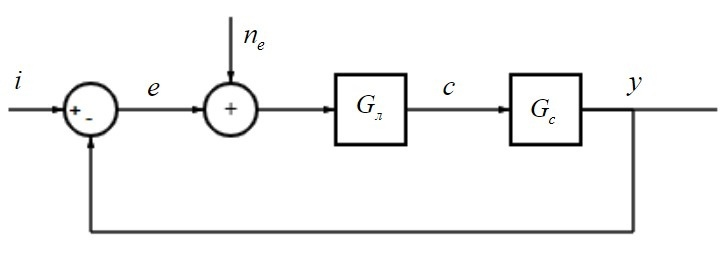
\includegraphics[width = \linewidth]{Оглавление/Part3/figures/СамолётЛётчик.png}}
    {\label{fig:Самолёт-лётчик}}
    \caption{Структурная схема системы самолёт-лётчик}   
\end{figure}

Чтобы далее оперировать спектральными плотностями, необходимо ввести некоторую ястность в происходящее. 

\begin{enumerate}
    \item Корреляционная функция -- это функция, которая задаёт связь между одной функцией и другой $R_{xy}$
    $$R_{xy} = \lim_{T \to \infty} \frac{1}{2T} \int_{-T}^{T} x(t) y(t+\tau) dt$$
    \item Спектральная плотность -- это корреляционная функция приобразованная через ряд Фурье.
    $$S_{xy} = \int_{-\infty}^{\infty} R_{xy}e^{-j\omega p} dt$$
\end{enumerate}

% Ремнанта ($n_e$) -- это шумы вводимые лётчиков в систему управления. Определим её как функцию из рис. {\ref{fig:Самолёт-лётчик}}
% \begin{equation}
%     \label{eq:Ремнанта}
%     n_e = 
% \end{equation}

Далее определим спектральную плотность ремнанты 

\begin{equation}
    \label{eq:Спектральная плотность ремнанты}
    S_{n_e n_e} = \frac{S_{e_n e_n}}{|\Phi^2|} 
\end{equation}

А также спектральную плотность входного сигнала

\begin{equation}
    \label{eq:Спектральная плотность входного сигнала}
    S_{ii} = \frac{1}{2T}I(j \omega)I(-j \omega) = \frac{A_\text{к}^2}{2}T,
\end{equation}
где $I(j \omega) = \int_{-T}^{T} A_\text{к} \cos{\omega_\text{к}t} = T(a_\text{к} - b_\text{к}j) = \Delta_\text{к}T$

\subsubsection{Передаточные функции систему ДУ}

Зная систему дифференциальных уравнений ({\ref{eq:Линеаризованная моель СПС}}), найдём передаточные функции 

\begin{equation}
    \label{eq:ПФ по горизонтальной скорости СПС}
    \{ \frac{V_x}{\delta_\text{э}} \} = \frac{-0.4412p^3 - 2,011p^2 + 3.388p + 4.471}{p^4 + 1.063p^3 + 0.1784p^2 + 0.003833p + 3.424 \cdot 10^{-5}}
\end{equation}

\begin{equation}
    \label{eq:ПФ по вертикальной скорости СПС}
    \{ \frac{V_y}{\delta_\text{э}} \} = \frac{-12.39^3 - 0.3612p^2 + 33.29p + 0.06517}{p^4 + 1.063p^3 + 0.1784p^2 + 0.003833p + 3.424 \cdot 10^{-5}}
\end{equation}

\begin{equation}
    \label{eq:ПФ по угловой скорости тангажа СПС}
    \{ \frac{\omega_z}{\delta_\text{э}} \} = \frac{-0.5845p^3 - 0.4285p^2 - 0.006449p - 3.57 \cdot 10^{-20}}{p^4 + 1.063p^3 + 0.1784p^2 + 0.003833p + 3.424 \cdot 10^{-5}}
\end{equation}

\begin{equation}
    \label{eq:ПФ по углу наклона траектории}
    \{ \frac{\theta}{\delta_\text{э}} \} = \frac{-0.5845p^2 - 0.4285p - 0.006449}{p^4 + 1.063p^3 + 0.1784p^2 + 0.003833p + 3.424 \cdot 10^{-5}}
\end{equation}

\subsection{План исследований}
\subsubsection{Обратная динамики }
Обратная динамика вычислена через обратные связи как показанно на рис.\ref{fig:САУ_ОД}
\begin{figure}[H]
    \centering 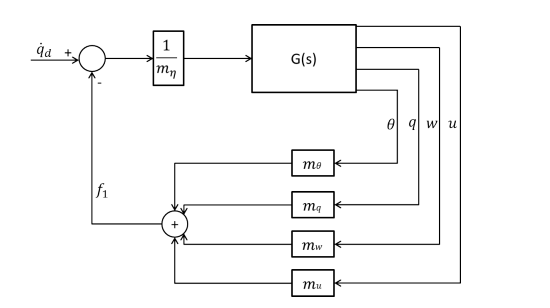
\includegraphics[width=15cm,height=10cm]{Оглавление/Part3/figures/Неполная схема СПС.png}
    \caption{Реализация динамической инверсии}
    {\label{fig:САУ_ОД}}
    \end{figure}
\subsection{Исследование робастности "Europe SPS"} 
\label{sec:Исследование робастности}

Чтобы изучить робастность "Europe SPS" необходимо воспользоваться моделью представленной на рис.{\ref{fig:Самолёт-лётчик}}

Результаты получаные при изучении робастности предоставлены на рис.\ref{fig:Модель без PI}

\begin{figure}[H]
    \centering 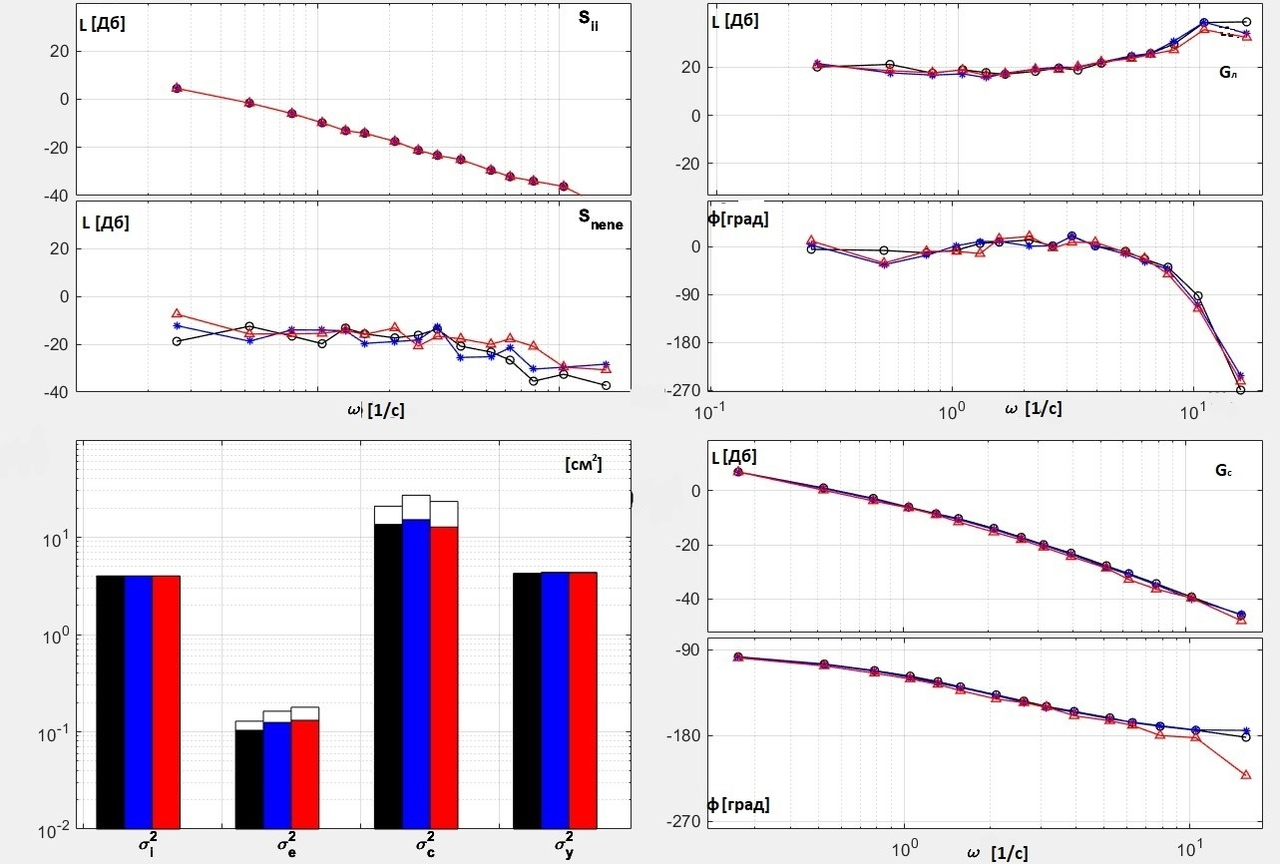
\includegraphics[width=\linewidth]{Оглавление/Part3/figures/Модель без PI.jpg}
    \caption{Результаты эксперимнтов без применения PI-контроллераы}
    {\label{fig:Модель без PI}}
\end{figure}
Из рис.{\ref{fig:Модель без PI}} видно, что с увеличением процнта неточности знаний лётчику сложнее выполнять задачу слежения 
(увеличивается разброс по ошибке $\sigma_e^2$)

\begin{table}[H]
    \caption{Результаты экспериментов}
    \centering
    \label{tab:Результаты экспериментов без PI}
    \begin{tabular}{|c|c|c|c|}
        \hline 
        № э.& $\sigma^2_e,$ см$^2$ & $\sigma^2_c$ см$^2$ & $n_e$ см$^2$ \\ \hline 
        1& 0.103 & 13.54 & 0.0254\\ \hline
        2& 0.125 & 15.14  & 0.037 \\ \hline
        3& 0.131 & 12.74 & 0.047\\ \hline

    \end{tabular}
\end{table}

\begin{table}[H]
    \caption{Результаты экспериментов}
    \centering
    \label{tab:Результаты экспериментов без PI2}
    \begin{tabular}{|c|c|c|c|c|}
        \hline 
        № э.&Нули & Полюса & $\xi$ & $\omega_c$, 1/c \\ \hline 
        1& -2 & - & 1.0 &0.5 \\ \hline
        & -1.9392 & -0.7537  &  & 1.59 $\cdot 10^{-4}$\\ 
        2& -0.7473 & -0.0161  &1.0 & 1.64 $\cdot 10^{-2}$\\ 
        & -0.0164 &  0 & &7.47 $\cdot 10^{-1}$\\ 
        & 0 &   &  &1.94 \\ \hline 
        & -1.8207 & 0.8255 & &0\\ 
        3& -0.8033 & -0.0177 & 1.0&1.85 $\cdot 10^{-2}$\\ 
        & -0.0185 & 0 & &8.03 $\cdot 10^{-1}$ \\ 
        & 0 &  &  &1.82 \\ \hline
    \end{tabular}
\end{table}


\begin{figure}[H]
    \centering 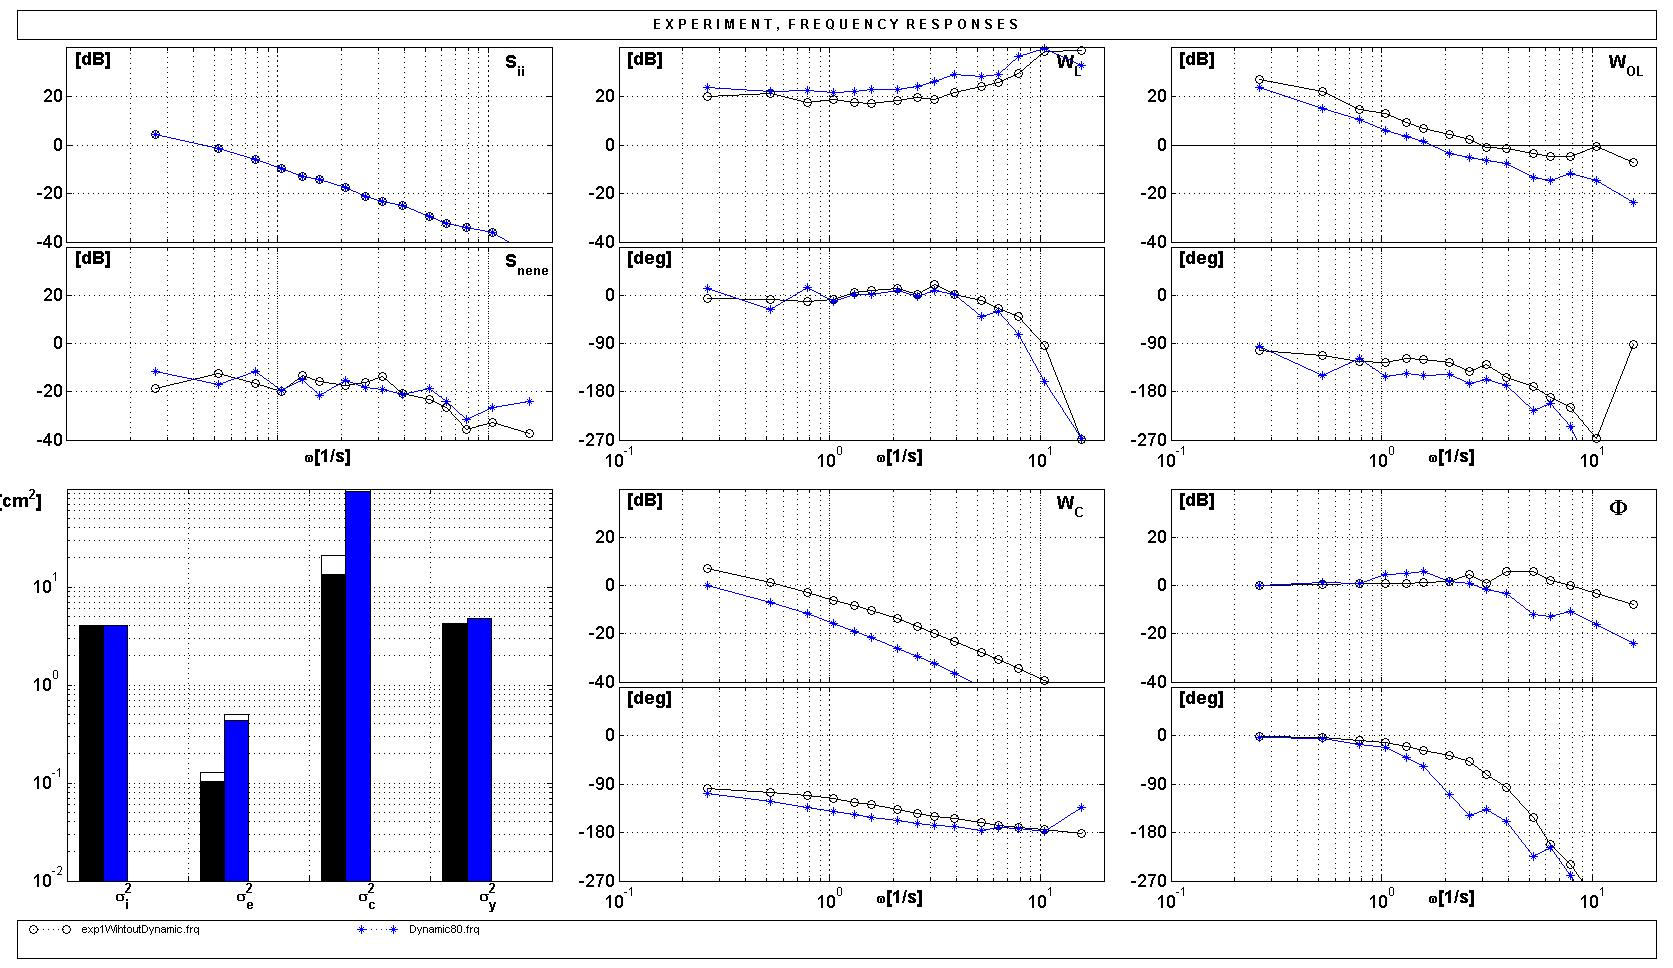
\includegraphics[width=\linewidth]{Оглавление/Part3/figures/testo2.jpg}
    \caption{Результаты эксперимнтов без применения PI-контроллераы}
    {\label{fig:Модель без PI 80}}
\end{figure}
Из рис. {\ref{fig:Модель без PI 80}} видно, что при увеличении неточности знаний --  разброс по ошибки значительно возрос, что
крайне затрудняет точно выполнять поствленную задачу слижения

\subsection{Улучшение робастности "Europe SPS"}
{\label{sec:Улучшение робастности}}

Как было показанно в разделе \ref{sec:Исследование робастности}, при введении обратной динамики -- 
значительно ухудшилось выполнение задачи компенсаторного слежения. Для улучшения робастности динамической системы с применением обратной
динамики в данной дипломной работе был выбран метод, который подразумеваем внедрение в систему управления PI-котроллера.

\begin{equation}
    \label{eq:PI}
    PI = K_p + \frac{1}{p}K_i = \frac{K_p p + K_i}{p},
\end{equation}


Результаты получаные при улучшении робастности с применением PI-контроллера предоставлены на рис.\ref{fig:Модель с PI}

\begin{figure}[H]
    \centering 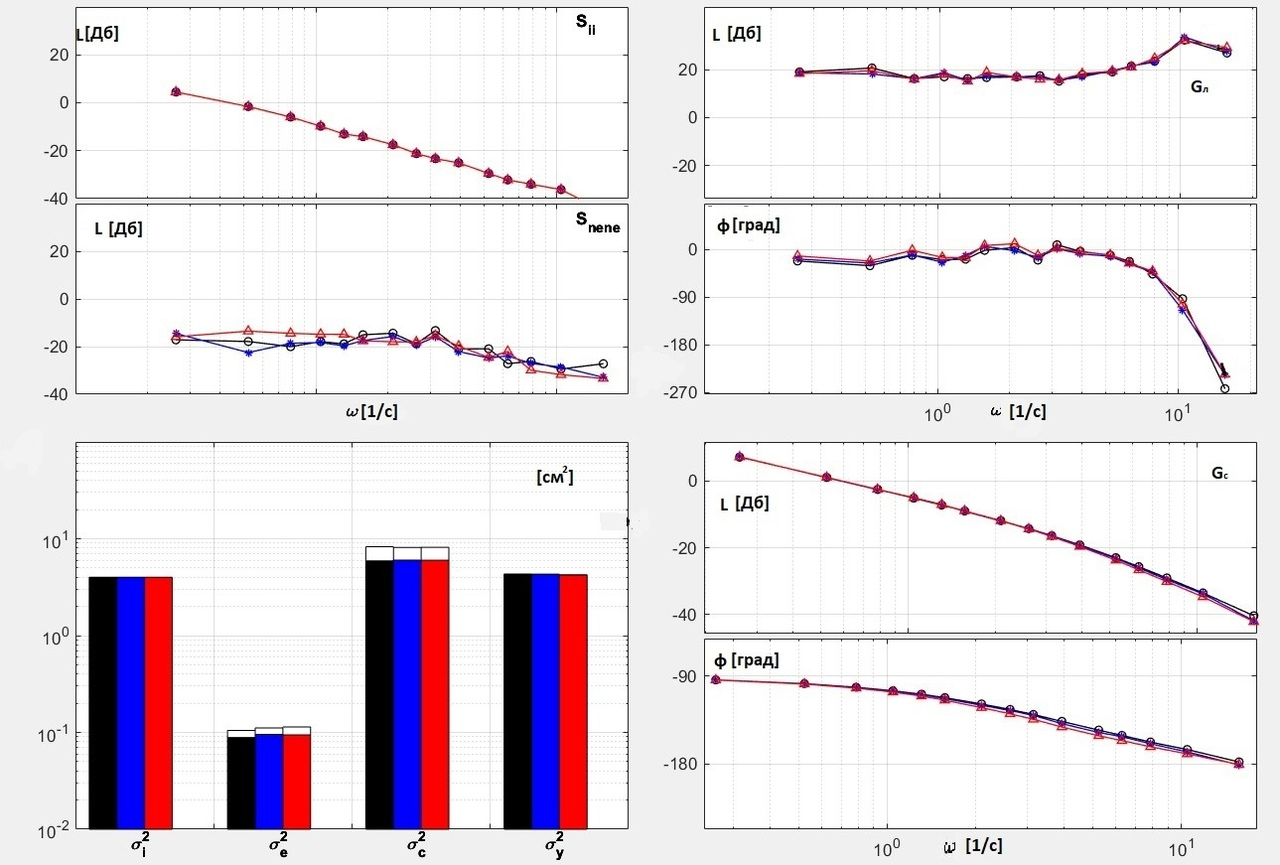
\includegraphics[width=\linewidth]{Оглавление/Part3/figures/Модель с PI.jpg}
    \caption{Результаты эксперимнтов c применения PI-контроллераы}
    \label{fig:Модель с PI}
\end{figure}


\begin{table}[H]
    \centering
    \caption{Результаты экспериментов}
    \begin{tabular}{|c|c|c|c|}
        \hline 
        № э.& $\sigma^2_e,$ см$^2$ & $\sigma^2_c$ см$^2$ & $n_e$ см$^2$ \\ \hline 
        1& 0.0886 & 5.913 & 0.01611\\ \hline
        2& 0.0952 & 6.01  & 0.01591 \\ \hline
        3& 0.0943 & 6.004 & 0.01712\\ \hline

    \end{tabular}
\end{table}
\end{frame}

\begin{table}[H]
    \centering
    \caption{Результаты расчётов}
    \label{tab:Результаты экспериментов PI}
    \begin{tabular}{|c|c|c|c|c|}
        \hline 
        № э.&Полюса & Нули & $\xi$ & $\omega_c$, 1/c \\ \hline 
        1& -3.0000 + 1.0000$i$ & -2.5 & 0.95 & 3.16\\ 
        & -3.0000 - 1.0000$i$ &   &  &  \\ \hline
        2& -2.8660 + 1.1287$i$ & -0.0161  & 1.0 &  0\\ 
        & -2.8660 - 1.1287$i$ &  -0.7537 &1.0 & 1.61$\cdot 10^{-2}$\\ 
        & -0.7547 + 0.0000$i$ &  -2.5000 & 1.0 & 7.51 $\cdot 10^{-2}$\\ 
        & 0 & 0.0000 & 0.93& 3.08 \\ 
        & -0.0161 + 0.0000$i$ &  & 0.93 &  \\ \hline 
        3& -2.5975 + 1.3096$i$ & -0.0177 & 1 & 0\\ 
        & -2.5975 - 1.3096$i$ & -0.8255 & 1& 1.77 $\cdot 10^{-2}$ \\ 
        & -0.8292 + 0.0000$i$ & -2.5000 & 1 & 8.29 $\cdot 10^{-1}$\\ 
        & 0 & 0 & 0.893 & 2.91 \\ 
        & -0.0177 + 0.0000$i$ &  &  &  \\ \hline 
    \end{tabular}
\end{table}


    \centering 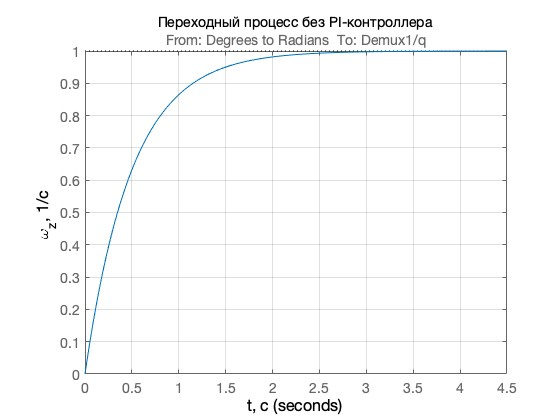
\includegraphics[width=\linewidth]{Оглавление/Part3/figures/withoutPI.jpg}
    \centering 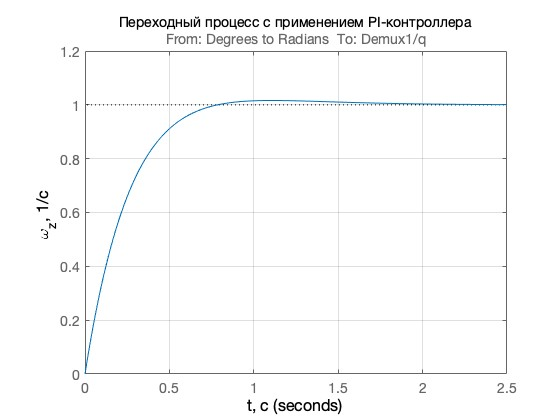
\includegraphics[width=\linewidth]{Оглавление/Part3/figures/withPI.jpg}

\begin{center}
    Выводы по разделу:
\end{center}
\begin{itemize}
    \item [] PI - котроллер за счёт того, что в его структуре имеется интегрирующее звено, по свойству интеграла, 
    сумирует бесконечно малые прирощения, в результате чего функция ошибки стремиться к нулю.
    \item [] Также можно наблюдать, что с введением в систему PI-котроллеру у системы появилось относительное перерегулирование, в результате чего, 
    время сробатывания уменьшилось, что благоприятно сказывается на решение задачи компенсаторного слежения.
    \item [] По корням характерестического уравнения \{$\frac{\omega_z}{\delta_\text{э}}$\}, можно сказать, что с введением PI- контроллера характериные корни начали сдвигаться
    к границам правой полуплоскости, это говорит о том, что система теряет устойчивость

\end{itemize}


    Также мы подразумеваем, что мы имеем дело с $K_\text{ш} = -0,6$
